\documentclass[a4paper]{article}

\usepackage[utf8]{inputenc}
\usepackage[spanish]{babel}

\usepackage[top=2cm, bottom=1.5cm, right=1.5cm, left=2cm]{geometry}

% \pagestyle{headings} %encabezado y pie sencillo

\usepackage{fancyhdr}
\pagestyle{fancy}

\setlength{\headheight}{13.6pt}

\lfoot[Data Science]{Data Science}
\rfoot[Proyecto Final]{Proyecto Final}

\usepackage{graphicx}
\graphicspath{ {images/} }%insertar imágenes

\usepackage{hyperref}%Links
\hypersetup{  %formato link
    colorlinks=true,
    linkcolor=blue,
    filecolor=blue,      
    urlcolor=blue,
    pdftitle={Data Science - Primer entrega del proyecto final},
    pdfpagemode=FullScreen,
    } 

\usepackage{float} %para fijar tablas
\usepackage{multirow} %Para tablas

\usepackage{booktabs}%para \toprule \midrule

\usepackage{ltablex}% para dividir tablas

% \usepackage{lscape} %para poner en horizontal una única hoja
\usepackage{pdflscape}

\usepackage{longtable}

\title{Curso Data Science \\ \vspace{0.5cm} Segunda entrega del proyecto final\\ \vspace{0.5cm}
Análisis socioeducativo de los habitantes de la Ciudad de Buenos Aires}

\author{Lucia Buzzeo, Lucia Hukovsky,\\ Jose Saint German, Juan Martín Carini}

\date{18 de agosto del 2022}

\begin{document}

\maketitle

\begin{center}
    
\includegraphics{Coder.png}
\end{center}

\thispagestyle{empty}

\newpage

\tableofcontents

\newpage

\section{Presentación del problema y fuente de información}

    \subsection{Presentación del problema}

        Nos es de gran de interés vivir en una comunidad con políticas públicas eficaces que mejoren las condiciones de vida de las personas. En este sentido, hemos decidido analizar los diferentes ejes que en nuestro país se rigen por políticas publicas. Al respecto, encontramos una gran limitación en el eje de educación al reconocer que su acceso dista de ser equitativo. Este aspecto no nos resultó una novedad, sin embargo, nos dio el pie para comenzar una investigación que permita dar una explicación teórica a la problemática. 
        En concreto, nos ha permitido conocer mejor la situación educativa actual de CABA y descubrir las principales variables que afectan el nivel educativo.
        
        El análisis realizado en el marco del presente proyecto podría establecer una base de requerimientos que permitan generar políticas públicas efectivas, no solo en el ámbito educativo, sino en el económico, cultural, social y geográfico, entre otros.

        \subsection{Definición de la fuente de información}

        Para trabajar esta problemática, hemos decidido recurrir a la \href{https://www.estadisticaciudad.gob.ar/eyc/?page_id=702}{datos abiertos} del Gobierno de la Ciudad de Buenos Aires para el año 2019. El mismo está disponible en la base de \href{https://data.buenosaires.gob.ar/dataset/encuesta-anual-hogares/resource/3a45c563-396d-42de-ba93-8a93729e0723}{Encuesta Anual de Hogares} del GCBA.

        Esta encuesta contiene información demográfica, social, económica, educativa y de salud de 14319 habitantes de la Ciudad, la cual es una muestra representativa que permite obtener un vistazo de la población de la Ciudad.

\newpage

\section{Pregunta y objetivos de investigación}

    Nuestro objetivo principal es descubrir las principales variables intervinientes en el nivel máximo educativo alcanzado por la población de la Ciudad Autónoma de Buenos Aires (CABA).

    De este objetivo principal se desprenden los siguientes sub-objetivos:
    \begin{itemize}
        \item Determinar si la ubicación geográfica del encuestado es determinante para alcanzar ciertos niveles educativos. De este objetivo se desprende determinar la relación entre el nivel educativo y la comuna del encuestado, así como la relación entre la misma variable y el hecho de que el encuestado habite en una villa de emergencia.
        \item Establecer la fuerza con la que el nivel socio-económico afecta la variable target.
        \item Explorar la relación del target con otras variables, como el sexo del encuestado, la cantidad de hijos, la afiliación de salud o la edad.
    \end{itemize}

\newpage

\section{Orden de trabajo}

    Este trabajo estará divido en 3 partes:
    \begin{enumerate}
        \item \textbf{Introducción a las variables del problema:} Se hará un análisis de las variables en donde se buscará conocer su performance dentro del dataset y su potencial signifícanos para la pregunta que buscamos responder. A la vez, queremos ver cómo las variables interactúan entre si. Esta parte es lo que se conoce como análisis univariado, bivariado y multivariado,
        \item \textbf{Modelos analíticos:} En esta sección se llevarán a cabo diversos modelos analíticos y algoritmos que nos servirán para acercarnos a la respuesta a nuestra pregunta de investigación,
        \item \textbf{Conclusión:} Haremos conclusiones finales sobre nuestros hallazgos. Además, discutiremos posibles limitaciones que tuviera y plantearemos futuras líneas de análisis a partir del análisis presente.
    \end{enumerate}

\newpage

\section{Análisis exploratorio de datos (EDA)}

    Una ves cargado el dataset con el que vamos a trabajar, miramos sus variable, el tipo que son y si tienen nulos:
    \begin{table}[H]\begin{center}
    \begin{tabular}{clll}
    \multicolumn{4}{l}{RangeIndex: 14319 entries, 0 to 14318} \\
    \multicolumn{4}{l}{Data columns (total 31 columns):}  \\
    \#  & Column                     & Non-Null Count & Dtype \\ \hline
    0  & id                          & 14319 non-null & int64 \\ 
    1  & nhogar                      & 14319 non-null & int64 \\ 
    2  & miembro                     & 14319 non-null & int64 \\ 
    3  & comuna                      & 14319 non-null & int64 \\ 
    4  & dominio                     & 14319 non-null & object \\
    5  & edad                        & 14319 non-null & int64 \\ 
    6  & sexo                        & 14319 non-null & object \\
    7  & parentesco\_jefe             & 14319 non-null & object \\
    8  & situacion\_conyugal          & 14318 non-null & object \\
    9  & num\_miembro\_padre           & 14319 non-null & object \\
    10 & num\_miembro\_madre           & 14319 non-null & object \\
    11 & estado\_ocupacional          & 14319 non-null & object \\
    12 & cat\_ocupacional             & 14319 non-null & object \\
    13 & calidad\_ingresos\_lab        & 14319 non-null & object \\
    14 & ingreso\_total\_lab           & 14319 non-null & int64  \\
    15 & calidad\_ingresos\_no\_lab     & 14319 non-null & object \\
    16 & ingreso\_total\_no\_lab        & 14319 non-null & int64  \\
    17 & calidad\_ingresos\_totales    & 14319 non-null & object \\
    18 & ingresos\_totales            & 14319 non-null & int64  \\
    19 & calidad\_ingresos\_familiares & 14319 non-null & object \\
    20 & ingresos\_familiares         & 14319 non-null & int64  \\
    21 & ingreso\_per\_capita\_familiar & 14319 non-null & int64  \\
    22 & estado\_educativo            & 14319 non-null & object \\
    23 & sector\_educativo            & 14316 non-null & object \\
    24 & nivel\_actual                & 14319 non-null & object \\
    25 & nivel\_max\_educativo         & 13265 non-null & object \\
    26 & años\_escolaridad            & 14257 non-null & object \\
    27 & lugar\_nacimiento            & 14318 non-null & object \\
    28 & afiliacion\_salud            & 14315 non-null & object \\
    29 & hijos\_nacidos\_vivos         & 6535 non-null  & object \\
    30 & cantidad\_hijos\_nac\_vivos    & 14319 non-null & object \\
    \multicolumn{4}{l}{dtypes: int64(10), object(21)}  \\ 
    \multicolumn{4}{l}{memory usage: 3.4+ MB} \\
    \end{tabular}\end{center}
    \end{table}
        
    Luego, generamos diversas transformaciones de variables, así como la creación de la variable "Target", pues es la que usaremos para todo el análisis:
    \begin{itemize}
        \item creamos el target para nivel\_max\_educativo,
        \item remplazamos los valores de años\_escolaridad para que todos sean numéricos,
        \item la variable ``cantidad\_hijos\_nac\_vivos'' se puede pasar a numérica si se toma ``no corresponde'' como NAN,
        \item hay determinadas variables (comuna, id, hogar y miembro) que están como numéricas pero deberían ser categóricas,
        \item generamos la variable ``target'' como copia de ``Target'' para tener ambas versiones,
        \item pasamos la variable Target a one hot encoding,
        \item por último renombramos algunas variables para que sean más cortas.
    \end{itemize}

    Ahora, con el dataset ya acomodado, comenzamos analizándolo en su conjunto. El mimsmo tiene 14319 filas y 36 columnas. Miramos las nuevas modificaciones en las variable, el tipo que son y si tienen nulos:
    \begin{table}[H]\begin{center}
    \begin{tabular}{clll}
        \multicolumn{4}{l}{$<$class 'pandas.core.frame.DataFrame'$>$} \\
        \multicolumn{4}{l}{RangeIndex: 14319 entries, 0 to 14318} \\
        \multicolumn{4}{l}{Data columns (total 36 columns):} \\
        \#  & Column                     & Non-Null Count & Dtype \\ \hline
        0 & id                           & 14319 non-null & object \\
        1 & nhogar                       & 14319 non-null & object \\
        2 &  miembro                     & 14319 non-null & object \\ 
        3 &  comuna                      & 14319 non-null & object  \\
        4 &  edad                        & 14319 non-null & int64   \\
        6 &  sexo                        & 14319 non-null & object \\
        5 &  parentesco\_jefe             & 14319 non-null & object  \\
        6 &  situacion\_conyugal          & 14318 non-null & object  \\
        7 &  num\_miembro\_padre           & 14319 non-null & object  \\
        8 &  num\_miembro\_madre           & 14319 non-null & object  \\
        9 &  estado\_ocupacional          & 14319 non-null & object  \\
        10 &  cat\_ocupacional            & 14319 non-null & object  \\
        11 & calidad\_ingresos\_lab        & 14319 non-null & object  \\
        12 & ingreso\_total\_lab           & 14319 non-null & int64   \\
        13 & calidad\_ingresos\_no\_lab     & 14319 non-null & object  \\
        14 & ingreso\_total\_no\_lab        & 14319 non-null & int64   \\
        15 & calidad\_ingresos\_totales    & 14319 non-null & object  \\
        16 & ingresos\_totales            & 14319 non-null & int64   \\
        17 & calidad\_ingresos\_familiares & 14319 non-null & object  \\
        18 & ingresos\_familiares         & 14319 non-null & int64   \\
        19 & ing\_per\_cap\_familiar        & 14319 non-null & int64   \\
        20 & estado\_educativo            & 14319 non-null & object  \\
        21 & sector\_educativo            & 14316 non-null & object  \\
        22 & nivel\_actual                & 14319 non-null & object  \\
        23 & nivel\_max\_educativo         & 13265 non-null & object  \\
        24 & años\_escolaridad            & 14257 non-null & float64 \\
        25 & lugar\_nacimiento            & 14318 non-null & object  \\
        26 & afiliacion\_salud            & 14315 non-null & object  \\
        27 & hijos\_nacidos\_vivos         & 6535 non-null  & object  \\
        28 & cant\_hijos\_nac\_vivos        & 14319 non-null & int64   \\
        29 & sexo\_Varon                  & 14319 non-null & uint8   \\
        30 & dominio\_villas              & 14319 non-null & uint8   \\
        31 & target                      & 13223 non-null & object  \\
        32 & Target\_inicial              & 14319 non-null & uint8   \\
        33 & Target\_prim\_completo        & 14319 non-null & uint8   \\
        34 & Target\_sec\_completo         & 14319 non-null & uint8   \\
        35 & Target\_superior             & 14319 non-null & uint8   \\
        \multicolumn{4}{l}{dtypes: float64(1), int64(7), object(22), uint8(6)}  \\
        \multicolumn{4}{l}{memory usage: 3.4+ MB}
    \end{tabular}\end{center}
    \end{table}

    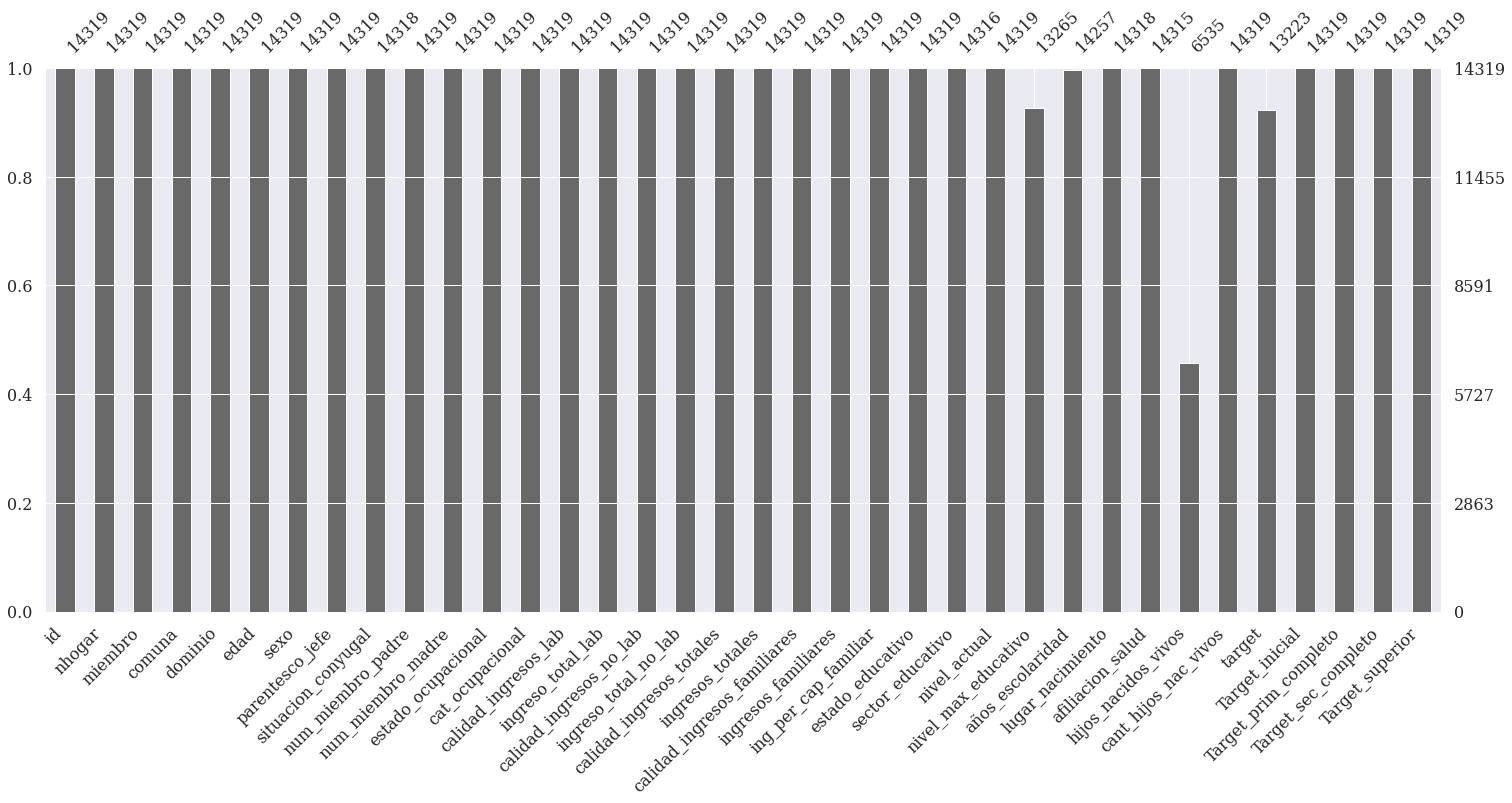
\includegraphics[scale=0.3]{GNulls.png}

    Tomamos el código visto en clase para tener un vistazo de las diversas medidas estadísticas de cada variable, donde calculamos información estadísticas y genéricas de cada columna en un dataframe:

    \begin{landscape}
    % \pagestyle{empty}
    \resizebox{24cm}{!} {
    \begin{tabular}{lllllllllllllllll}
        \toprule
        {} &                        index & Cantidad &     Tipo & Missing &  Unicos & Numeric &                            top &          mean &           std &  min &      25\% &      50\% &      75\% &        max &      sesgo &        kurt \\
        Etiqueta                                           &                              &          &          &         &         &         &                                &               &               &      &          &          &          &            &            &             \\
        \midrule
        Clave que identifica la vivienda                   &                           id &  14319.0 &   object &     0.0 &  5795.0 &   False &                           4291 &             - &             - &    - &        - &        - &        - &          - &    0.16901 &   -0.953158 \\
        La variable id + nhogar = clave que identifica ... &                       nhogar &  14319.0 &   object &     0.0 &     7.0 &   False &                              1 &             - &             - &    - &        - &        - &        - &          - &  21.366705 &  687.880709 \\
        Variables id + nhogar + miembro = clave que ide... &                      miembro &  14319.0 &   object &     0.0 &    19.0 &   False &                              1 &             - &             - &    - &        - &        - &        - &          - &   1.940715 &    8.605228 \\
        Comuna donde reside la persona encuestada          &                       comuna &  14319.0 &   object &     0.0 &    15.0 &   False &                              8 &             - &             - &    - &        - &        - &        - &          - &   0.103211 &   -1.090936 \\
        Edad de la persona encuestada                      &                         edad &  14319.0 &    int64 &     0.0 &   101.0 &    True &                              - &      38.81549 &      23.11017 &  0.0 &     20.0 &     37.0 &     57.0 &      100.0 &   0.249452 &   -0.868539 \\
        Sexo de la persona encuestada                      &                         sexo &  14319.0 &   object &     0.0 &     2.0 &   False &                          Mujer &             - &             - &    - &        - &        - &        - &          - &          - &           - \\
        Parentesco entre la persona encuestada y el jef... &              parentesco\_jefe &  14319.0 &   object &     0.0 &     9.0 &   False &                           Jefe &             - &             - &    - &        - &        - &        - &          - &          - &           - \\
        Situación conyugal de la persona encuestada        &           situacion\_conyugal &  14318.0 &   object &     1.0 &     7.0 &   False &                      Soltero/a &             - &             - &    - &        - &        - &        - &          - &          - &           - \\
        Número de miembro que corresponde al padre         &            num\_miembro\_padre &  14319.0 &   object &     0.0 &     9.0 &   False &                 No corresponde &             - &             - &    - &        - &        - &        - &          - &          - &           - \\
        Número de miembro que corresponde a la madre       &            num\_miembro\_madre &  14319.0 &   object &     0.0 &    11.0 &   False &                 No corresponde &             - &             - &    - &        - &        - &        - &          - &          - &           - \\
        Situación ocupacional de la persona encuestada     &           estado\_ocupacional &  14319.0 &   object &     0.0 &     3.0 &   False &                        Ocupado &             - &             - &    - &        - &        - &        - &          - &          - &           - \\
        Categoría ocupacional de la persona encuestada     &              cat\_ocupacional &  14319.0 &   object &     0.0 &     5.0 &   False &                 No corresponde &             - &             - &    - &        - &        - &        - &          - &          - &           - \\
        Calidad de la declaración de ingresos laborales... &         calidad\_ingresos\_lab &  14319.0 &   object &     0.0 &     4.0 &   False &  Tuvo ingresos y declara monto &             - &             - &    - &        - &        - &        - &          - &          - &           - \\
        Ingreso total laboral percibido el mes anterior    &            ingreso\_total\_lab &  14319.0 &    int64 &     0.0 &   440.0 &    True &                              - &   20078.62644 &  34698.173111 &  0.0 &      0.0 &   2500.0 &  30000.0 &  1000000.0 &   5.699235 &   81.275336 \\
        Calidad de la declaración de ingresos no labora... &      calidad\_ingresos\_no\_lab &  14319.0 &   object &     0.0 &     4.0 &   False &               No tuvo ingresos &             - &             - &    - &        - &        - &        - &          - &          - &           - \\
        Ingreso total no laboral percibido el mes anterior &         ingreso\_total\_no\_lab &  14319.0 &    int64 &     0.0 &   375.0 &    True &                              - &   6016.234583 &  16065.350052 &  0.0 &      0.0 &      0.0 &   4000.0 &   500000.0 &   6.889678 &  104.118617 \\
        Calidad de ingresos totales individuales           &     calidad\_ingresos\_totales &  14319.0 &   object &     0.0 &     4.0 &   False &  Tuvo ingresos y declara monto &             - &             - &    - &        - &        - &        - &          - &          - &           - \\
        Ingreso total individual percibido el mes anterior &             ingresos\_totales &  14319.0 &    int64 &     0.0 &   678.0 &    True &                              - &  26094.861024 &  37152.503186 &  0.0 &      0.0 &  16000.0 &  37000.0 &  1000000.0 &   5.333472 &   68.292205 \\
        Calidad de ingresos totales familiares             &  calidad\_ingresos\_familiares &  14319.0 &   object &     0.0 &     3.0 &   False &  Tuvo ingresos y declara monto &             - &             - &    - &        - &        - &        - &          - &          - &           - \\
        Ingresos totales familiares percibido el mes an... &          ingresos\_familiares &  14319.0 &    int64 &     0.0 &   960.0 &    True &                              - &  70212.818423 &  62685.684278 &  0.0 &  30000.0 &  54000.0 &  90000.0 &  1000000.0 &   3.312553 &   20.475526 \\
        Ingreso familiar per capita percibido el mes an... &         ing\_per\_cap\_familiar &  14319.0 &    int64 &     0.0 &  1257.0 &    True &                              - &  26192.009638 &  27463.908496 &  0.0 &  10500.0 &  19900.0 &  33500.0 &  1000000.0 &   6.970584 &  145.623563 \\
        Asistencia (pasada o presente) o no a algún est... &             estado\_educativo &  14319.0 &   object &     0.0 &     3.0 &   False &         No asiste pero asistió &             - &             - &    - &        - &        - &        - &          - &          - &           - \\
        Sector al que pertenece el establecimiento educ... &             sector\_educativo &  14316.0 &   object &     3.0 &     4.0 &   False &                 No corresponde &             - &             - &    - &        - &        - &        - &          - &          - &           - \\
        Nivel cursado al momento de la encuesta            &                 nivel\_actual &  14319.0 &   object &     0.0 &    14.0 &   False &                 No corresponde &             - &             - &    - &        - &        - &        - &          - &          - &           - \\
        Máximo nivel educativo que se cursó                &          nivel\_max\_educativo &  13265.0 &   object &  1054.0 &     7.0 &   False &         Secundario/medio comun &             - &             - &    - &        - &        - &        - &          - &          - &           - \\
        Años de escolaridad alcanzados                     &             años\_escolaridad &  14257.0 &  float64 &    62.0 &    20.0 &    True &                              - &     10.907905 &      5.353943 &  0.0 &      7.0 &     12.0 &     15.0 &       19.0 &  -0.624452 &   -0.517683 \\
        Lugar de nacimiento de la persona encuestada       &             lugar\_nacimiento &  14318.0 &   object &     1.0 &     7.0 &   False &                           CABA &             - &             - &    - &        - &        - &        - &          - &          - &           - \\
        Afiliación de salud de la persona encuestada       &             afiliacion\_salud &  14315.0 &   object &     4.0 &     5.0 &   False &               Solo obra social &             - &             - &    - &        - &        - &        - &          - &          - &           - \\
        Tiene o tuvo hijos nacidos vivos                   &          hijos\_nacidos\_vivos &   6535.0 &   object &  7784.0 &     2.0 &   False &                             Si &             - &             - &    - &        - &        - &        - &          - &          - &           - \\
        Cantidad de hijos nacidos vivos                    &         cant\_hijos\_nac\_vivos &  14319.0 &    int64 &     0.0 &    14.0 &    True &                              - &      0.630072 &      1.217323 &  0.0 &      0.0 &      0.0 &      1.0 &       15.0 &   2.560422 &    9.774595 \\
        ¿El encuestado es varón? no:0, si:1                &                   sexo\_Varon &        - &        - &       - &       - &       - &                              - &             - &             - &    - &        - &        - &        - &          - &          - &           - \\
        ¿El encuestado vive en una villa de emergencia?... &               dominio\_villas &        - &        - &       - &       - &       - &                              - &             - &             - &    - &        - &        - &        - &          - &          - &           - \\
        Nivel máximo educativo                             &                       target &  13223.0 &   object &  1096.0 &     4.0 &   False &                   sec\_completo &             - &             - &    - &        - &        - &        - &          - &          - &           - \\
        Nivel inicial                                      &               Target\_inicial &  14319.0 &    uint8 &     0.0 &     2.0 &    True &                              - &      0.107549 &      0.309821 &  0.0 &      0.0 &      0.0 &      0.0 &        1.0 &   2.533754 &    4.420525 \\
        Nivel primaro completo                             &         Target\_prim\_completo &  14319.0 &    uint8 &     0.0 &     2.0 &    True &                              - &       0.21908 &      0.413637 &  0.0 &      0.0 &      0.0 &      0.0 &        1.0 &   1.358484 &   -0.154543 \\
        Nivel secundario completo                          &          Target\_sec\_completo &  14319.0 &    uint8 &     0.0 &     2.0 &    True &                              - &      0.417348 &      0.493138 &  0.0 &      0.0 &      0.0 &      1.0 &        1.0 &   0.335257 &   -1.887867 \\
        Nivel superior                                     &              Target\_superior &  14319.0 &    uint8 &     0.0 &     2.0 &    True &                              - &      0.179482 &      0.383769 &  0.0 &      0.0 &      0.0 &      0.0 &        1.0 &   1.670605 &    0.791033 \\
        -                                                  &                      dominio &  14319.0 &   object &     0.0 &     2.0 &   False &             Resto de la Ciudad &             - &             - &    - &        - &        - &        - &          - &          - &           - \\
        \bottomrule
    \end{tabular} }
    \end{landscape}
               
    Y detectamos que nuestra variable target tiene 1054 valores nulos. Es importante tener este dato presente cuando querramos correr un algoritmo de clasificación.
    
    \subsection{Análisis univariado}
    
        \subsubsection{Género y edad}
        
            Comenzamos con un pantallazo general sobre las primeras cualidades de los datos, como muestra representativa para la EPH, sobre quiénes son los ciudadanos representado en el dataset.
        
            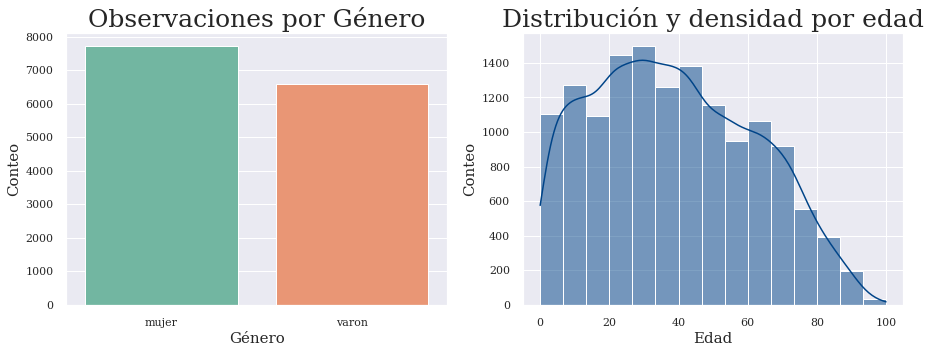
\includegraphics[scale=0.5]{GGenYEdad.png}

            En la variable género los datos parecen equilibrados en las categorías. Para el caso de la variable "edad", la distribución se asemeja a la de una normal.
        
        \subsubsection{Comuna}
        
            Seguimos observando la variable ``comuna". En la misma se muestra la comuna de la Ciudad de Buenos Aires del entrevistado, de manera de tener una ubicación geográfica. Consideramos importante revisar esta variable ya que tenemos como hipótesis que el nivel educativo alcanzado puede estar dependiendo de la zona geográfica de la ciudad en la que se encuentra el entrevistado.
        
            Para esto vamos a generar un mapa, así que utilizaremos el mapa de comunas de la Ciudad de Buenos Aires, transformamos las variables que vamos a usar para joinear el mapa con la base de manera que coincidan, transformamos la base para contablizar la frecuencia con la que aparece cada comuna en la base. Y por último unimos ambos datasets y generamos una nueva variable con las coordenadas para poder agregar etiquetas en el centro geográfico de cada comuna, que nos da como resultado los siguientes graficos:
        
            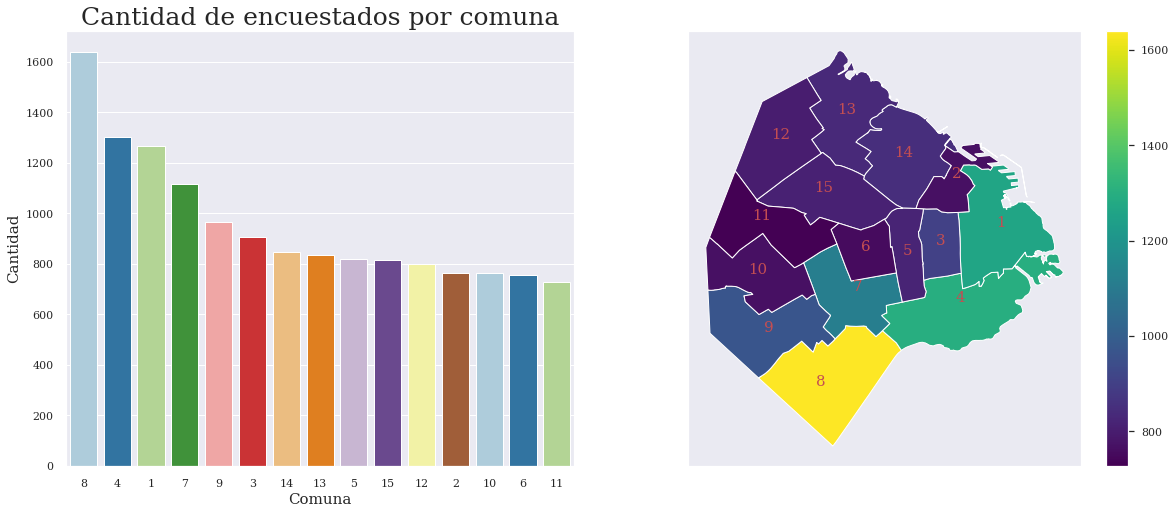
\includegraphics[scale=0.4]{GComuna1.png}

            Observando ambos gráficos vemos que las comunas 1,4,7 y 8 tienen mayor cantidad de casos. Queda por verse si en posteriores análisis es necesario abordar esta diferencia para evitar sesgos. Para eso, será necesario tomar en cuenta el porcentaje de la población total de cada comuna.
        
        \subsubsection{Ingreso familiar per capita}
        
            Ahora probamos con observar los ingresos familiares. Creemos que puede ser un indicador interesante del nivel educativo.
        
            Para esto, armamos una función para graficar y jugar con el nivel del filtrado de la variable y obtener un histograma que permita apreciar mejor la distribución de la variable sin tantos outliers. Probamos graficando con el máximo de la variable:
        
            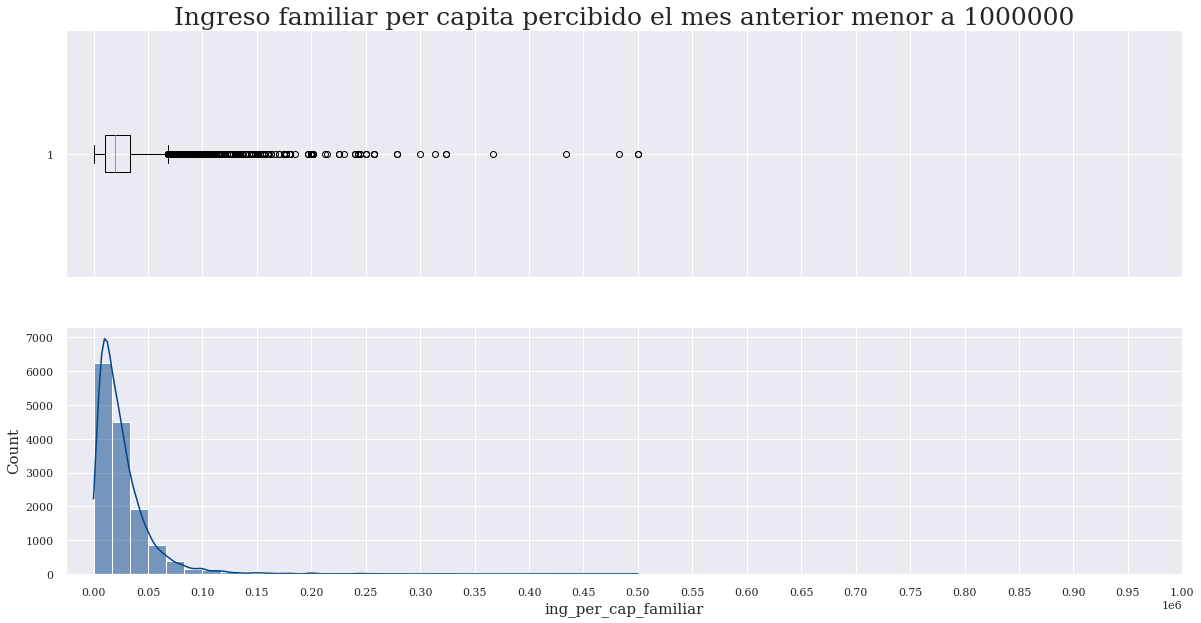
\includegraphics[scale=0.4]{GIFPC1.png}
        
            Y como hay muchos outliers que impiden ver la distribución correctamente, los quitamos de los gráficos:
        
            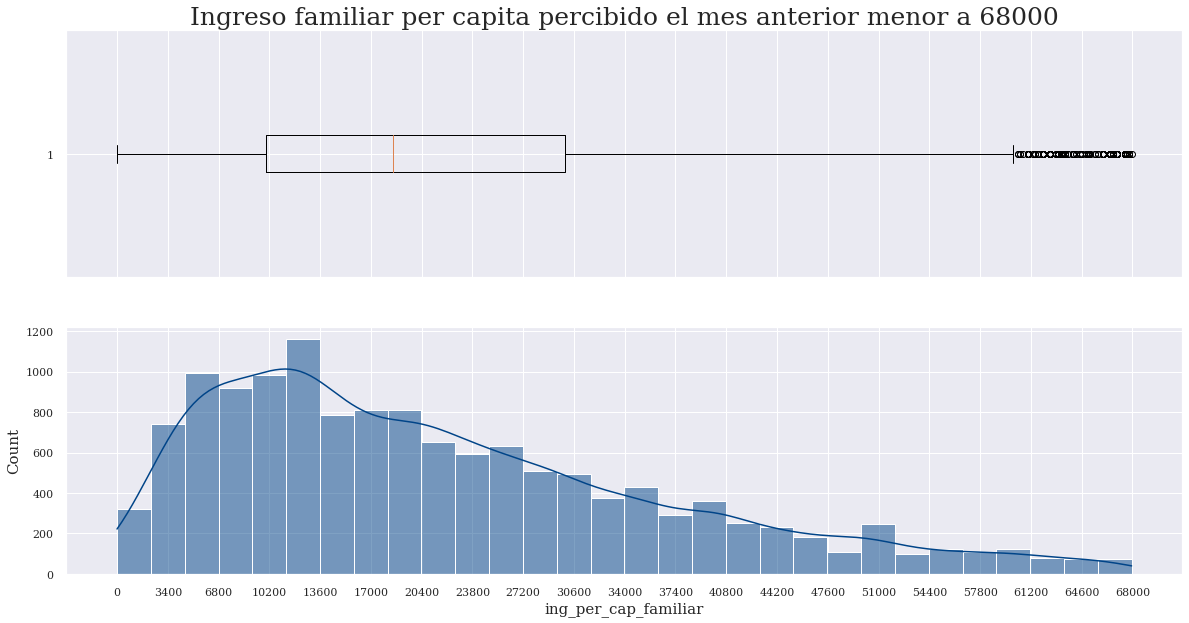
\includegraphics[scale=0.4]{GIFPC2.png}

            De este forma vemos que, aún removiendo los outliers, la distribución sigue sesgada.

        \newpage    

        \subsubsection{Años de escolaridad}
        
            Analizamos mediante un gráfico de barras los años de escolaridad alcanzados por los encuestados:
            
            \includegraphics[scale=0.7]{GAñosEsc.png}
            
            A simple vista se observan tres "picos": en el valor mínimo, alrededor del 7.5 y alrededor del 12.5. Podemos inferir que estos tres casos corresponden a no tener estudios, solo haber transcurrido el primario y haber transcurrido hasta la educación secundaria, respectivamente.
        
        \subsubsection{Máximo nivel educativo (Target)}
        
            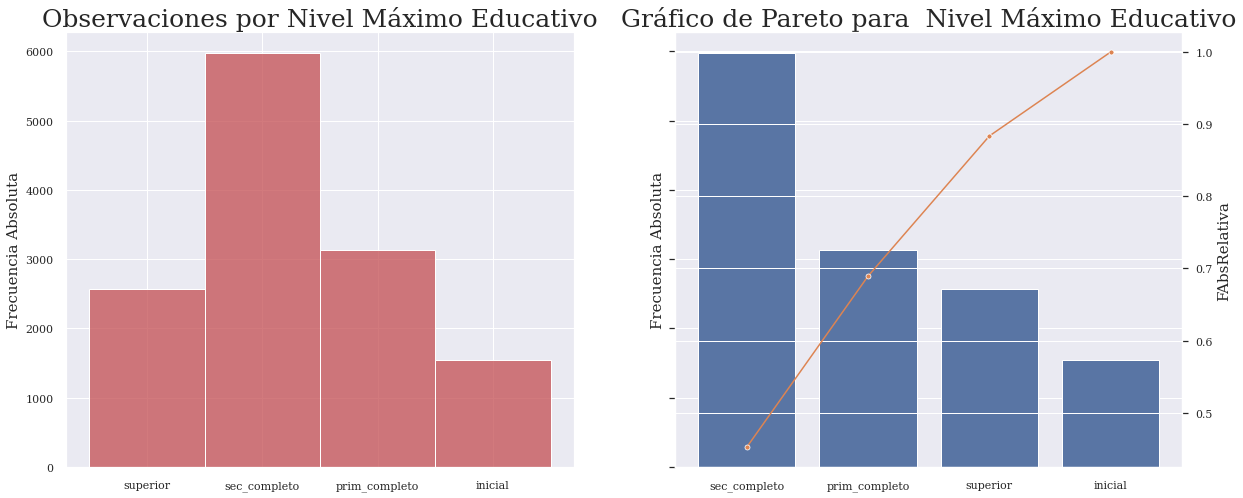
\includegraphics[scale=0.35]{GMNEA.png}
        
            Podemos observar que el nivel máximo educativo más alcanzado es el secundario completo, seguido por el primario. Contrario de lo que habíamos intuido anteriormente, el nivel superior quedó en tercer lugar. Adicionalmente, el nivel secundario y primario explican casi el 77\% de los datos.

    \newpage

    \subsection{Análisis bivariado}

        Realizamos diferentes heatmaps para ver si algo nos llama la atención, utilizando el método de correlación de Spearman:

        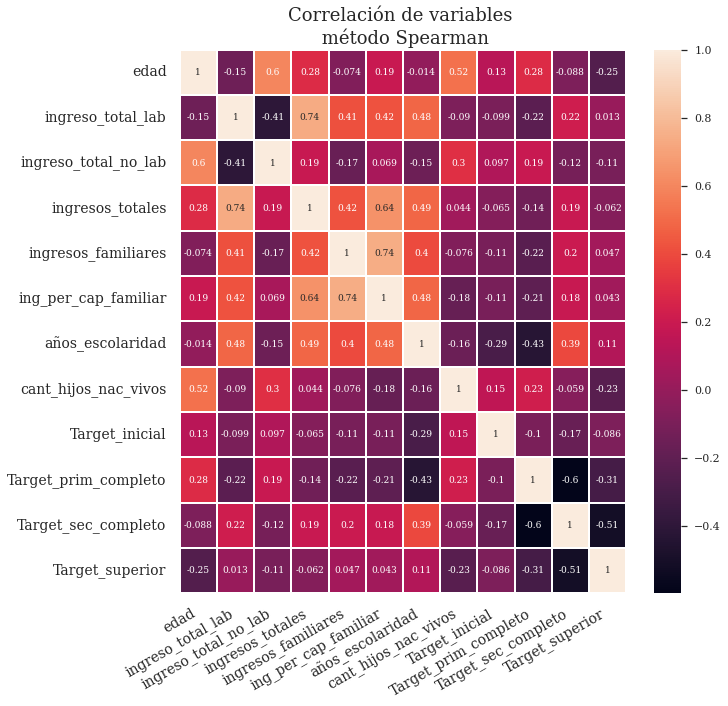
\includegraphics[scale=0.6]{GHitMap1.png}

        A simple vista, no se observan fuertes correlaciones. Sorprende la relación entre la variable sexo\_Varon y el resto. Convendría consultar con el profesor para saber qué puede estar ocurriendo.

        Podemos notar que en la variable que habíamos elegido como target para clasificar por nivel educativo no muestra correlaciones fuertes con las demás variable. Sin embargo, su versión numérica (años\_escolaridad) si. La principal correlación positiva es años\_escolaridad con ingreso familiar per cápita (ing\_per\_cap\_familiar), lo cual hace sentido teórico. Adicionalmente, el ingreso familiar per capita tiene una correlación fuerte negativa con dominio\_villa.

        Graficar en base a un threshold de 0.6 y 0.5 de correlación:

        \begin{center}
            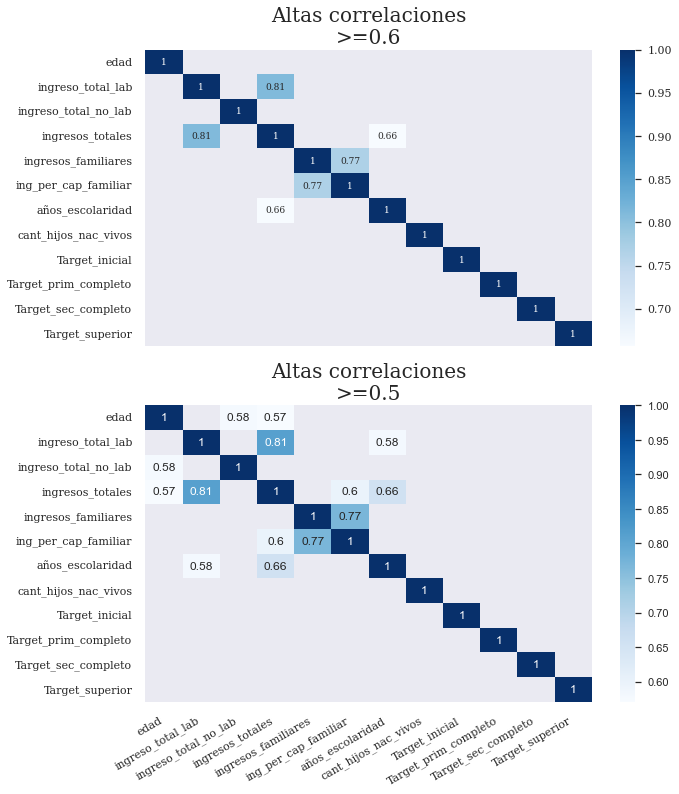
\includegraphics[scale=0.7]{GHitMap2.png}
        \end{center}

        Por último corremos una tabla de correlación y filtramos las de valores más altos:


        \begin{tabular}{lllr}
             & Variable\_1 & Variable\_2 & corr\_value \\
             3 & ingreso\_total\_lab & ingresos\_totales & 0.810840 \\
             7 & ingresos\_familiares & ing\_per\_cap\_familiar & 0.769356 \\
             6 & ingresos\_totales & años\_escolaridad & 0.656880 \\
             5 & ingresos\_totales & ing\_per\_cap\_familiar & 0.598997 \\
             4 & ingreso\_total\_lab & años\_escolaridad & 0.579614 \\
             1 & edad & ingreso\_total\_no\_lab & 0.578532 \\
             2 & edad & ingresos\_totales & 0.570521 \\
        \end{tabular}

    Conclusiones:
    \begin{itemize}
        \item Como es esperable, hay alta correlación entre las variables relacionadas al ingreso.
        \item A su vez, encontramos una alta correlación (66\%) entre los ingresos y los años de escolaridad.
        \item También observamos una relación positiva entre la edad y los ingresos totales.
        \item Por último, si bien no es tan alta como las demás correlaciones, parece que la cantidad de hijos nacidos vivos correlaciona negativamente con ser varón.
    \end{itemize}

        \subsubsection{Comparación entre variables numéricas}
        
        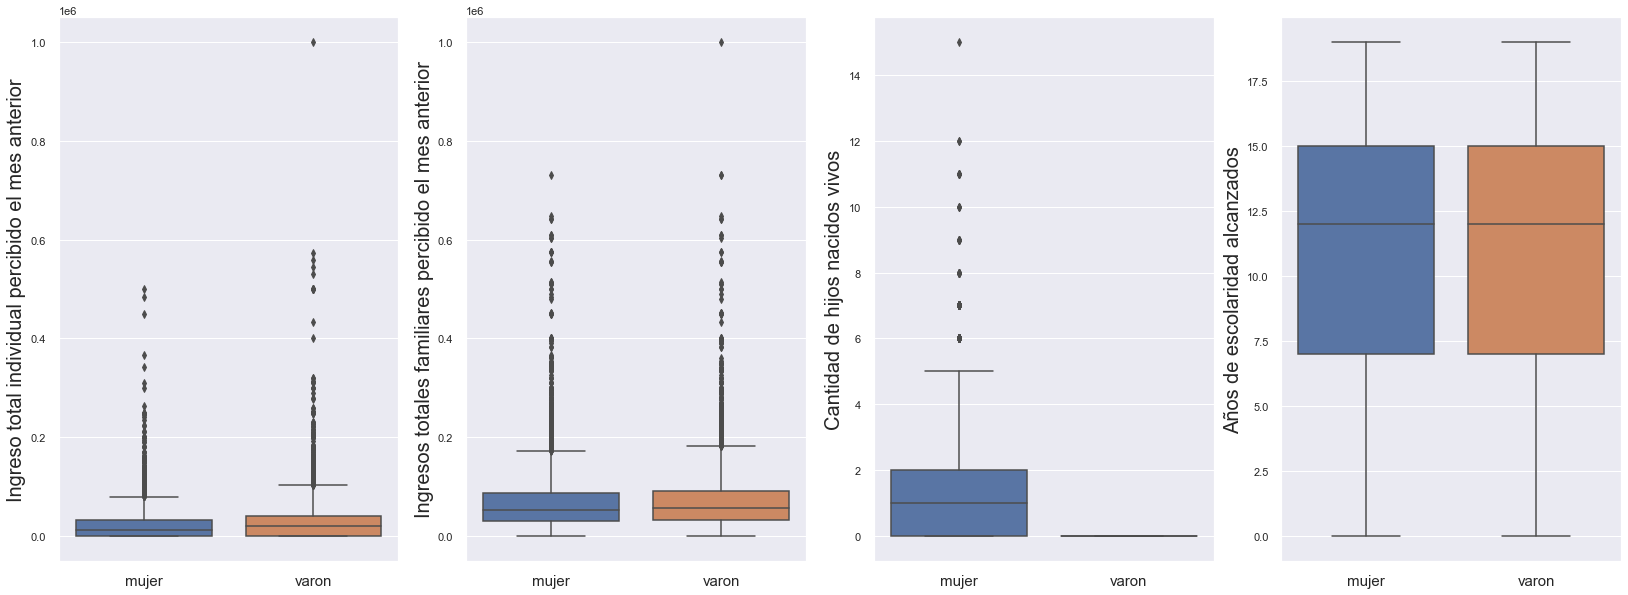
\includegraphics[scale=0.28]{GComVarNum1.png}

        Por parte de las variables de ingreso, no parece haber nada disruptivo. La distribución por ingreso y años de escolaridad pareciera ocurrir pero no en un orden lineal.

        Sigue llamando la atención la variable sexo\_Varon: por algún motivo, todos los encuestados hombres figuran sin hijos nacidos vivos. Alternativamente, se podría investigar la metodología de la encuesta para ver si hay alguna respuesta. Adicionalmente, los hombres parecieran tener ingresos totales y familiares mayores que las mujeres (sexo\_varon=0), pero no pareciera que haya distribuciones desiguales en los años de escolaridad.

        A continuación hacemos un gráfico lineal en base a la edad comparando el ingreso familiar con los ingresos totales. 

        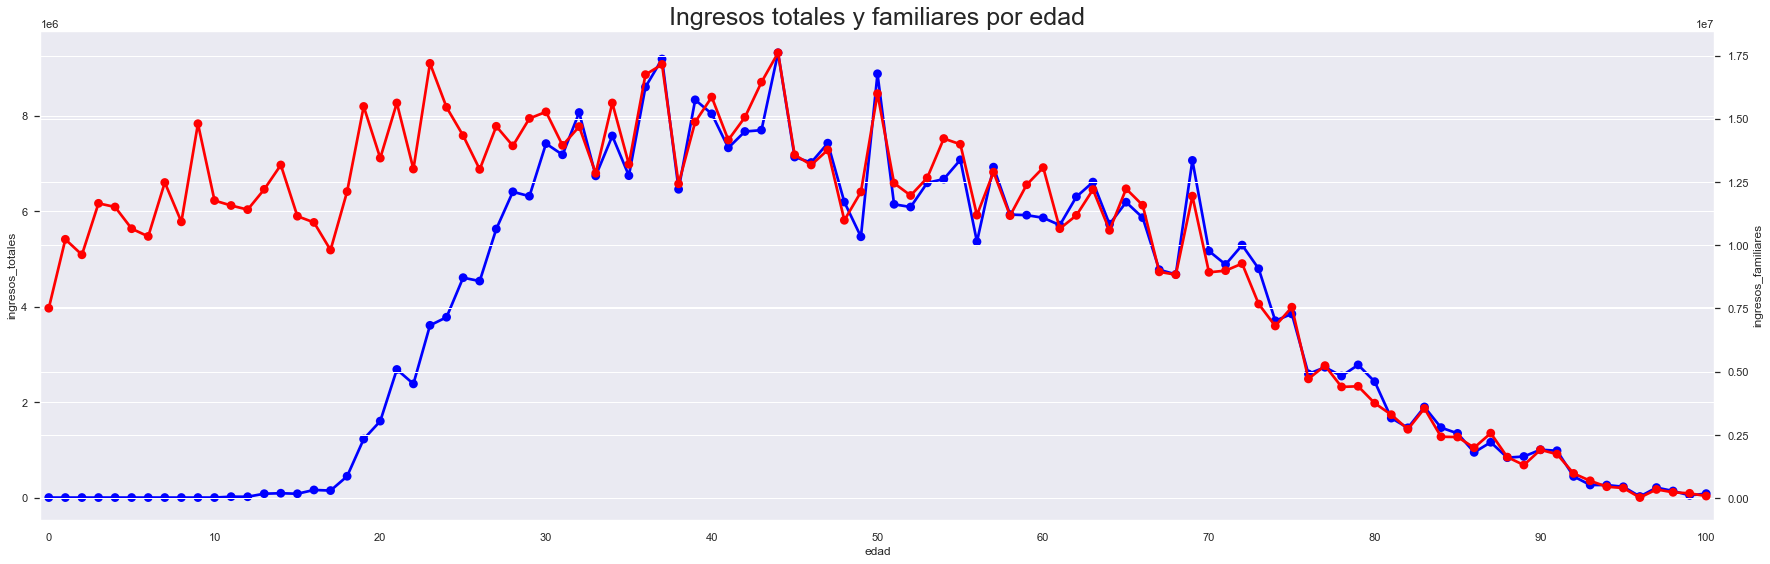
\includegraphics[scale=0.27]{GComVarNum2.png}

        Se puede ver que desde los 30 años en adelante el ingreso total de la persona se corresponde con el ingreso familiar. Por ende suele haber un único ingreso fuerte por grupo familiar.

        \newpage

        \subsubsection{Comparación de variables categóricas con numéricas}
        
        Adicionalmente, vamos a comparar algunas variables con nuestro target, comenzando con los ingresos totales:

        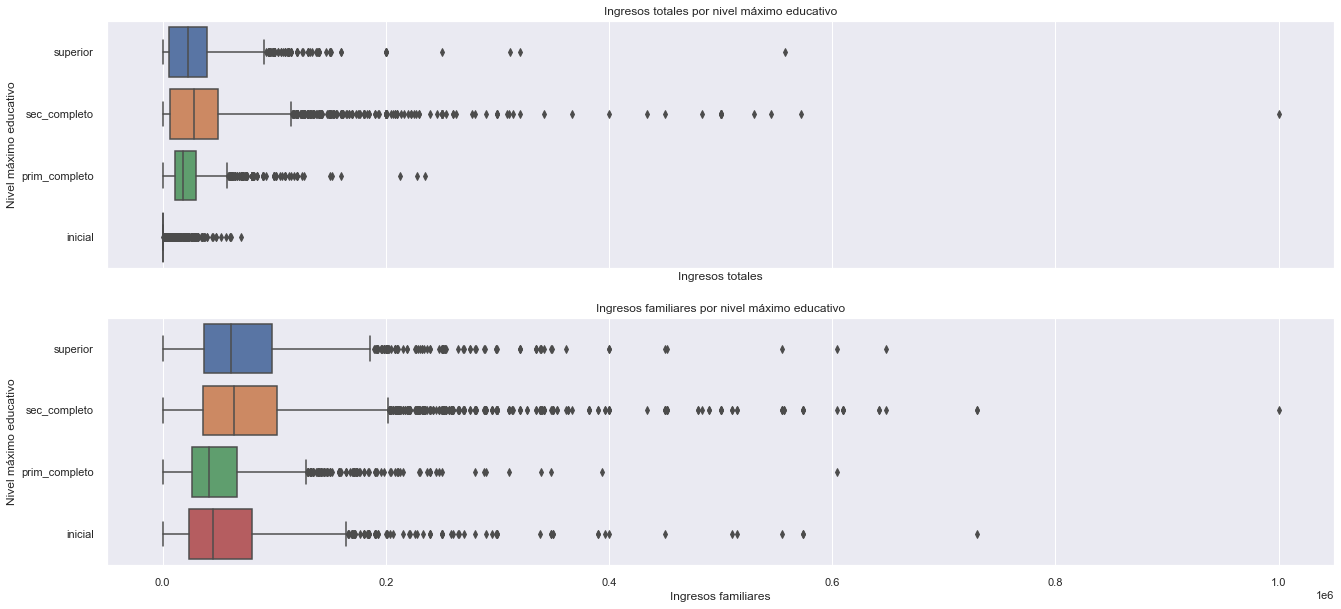
\includegraphics[scale=0.35]{GComVarCatNum1.png}
        
        \subsubsection{Variable numéricas con comuna}
        
        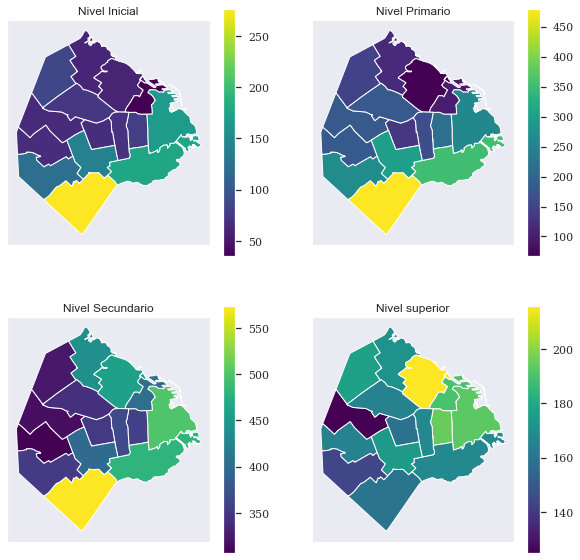
\includegraphics[scale=0.8]{GVarNumCom1.png}
        
        Se observa que en el sur de la ciudad hay mayor cantidad de encuestados con niveles de inicial, primario y secundario completo, mientras que el norte (particularmente el barrio de Palermo) tiene mayor cantidad de personas con estudios superiores. En menor medida también las comunas del este (comunmente llamado el "centro" de la ciudad) destacan por la cantidad de encuestados con nivel superior.
        
        \begin{center}
            \includegraphics[scale=0.9]{GAñosEscXCom.png}
        \end{center}

        Lo que podemos observar en los últimos dos gráficos es una clara división geográfica del nivel educativo.
        \begin{itemize}
            \item Las comunas del norte son las que tienen mayor nivel educativo.
            \item Las comunas del centro tienen niveles medios.
            \item Las comunas del sur (con las comuna 6 en el centro de la ciudad como outlier) y la comuna 1 en el este son las que tienen niveles más bajos.
        \end{itemize}
    
    \newpage
    
    \subsection{Análisis multivariado}
        
        \subsubsection*{Años de escolaridad, nivel máximo educativo e ingresos totales}

            Probamos de cruzar años de escolaridad, nivel máximo educativo y los ingresos totales.

            \begin{center}
                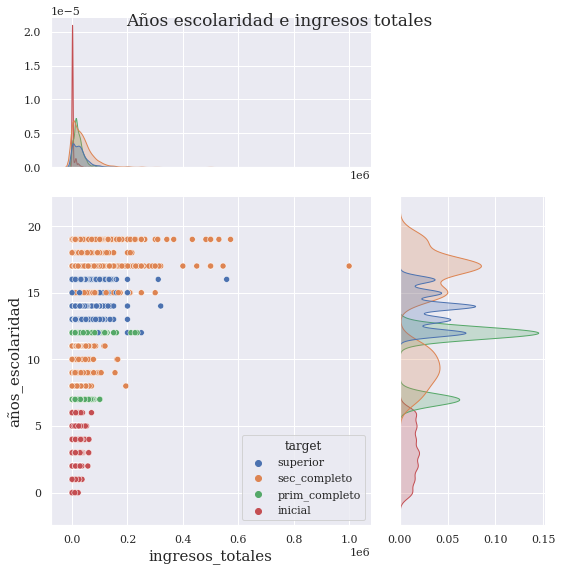
\includegraphics[scale=0.8
                ]{GMul1.png}
            \end{center}

            Conclusiones de la visualización:
            \begin{itemize}
                \item Hasta los 6 años, como era esperable, todos los casos llegan al nivel inicial.
                \item Vemos dos años en que aparece el primario completo: 7 y 12 años.Estimamos que se debe a la división entre los que comenzaro su educación en la primaria y los que comenzaron en el nivel inicial.
                \item A partir de los 12 años vemos un aumento consistente de los ingresos totales.
            \end{itemize}
        
        \begin{landscape}
            
        \subsubsection*{Ingresos familiares por el nivel máximo educativo y el dominio}

            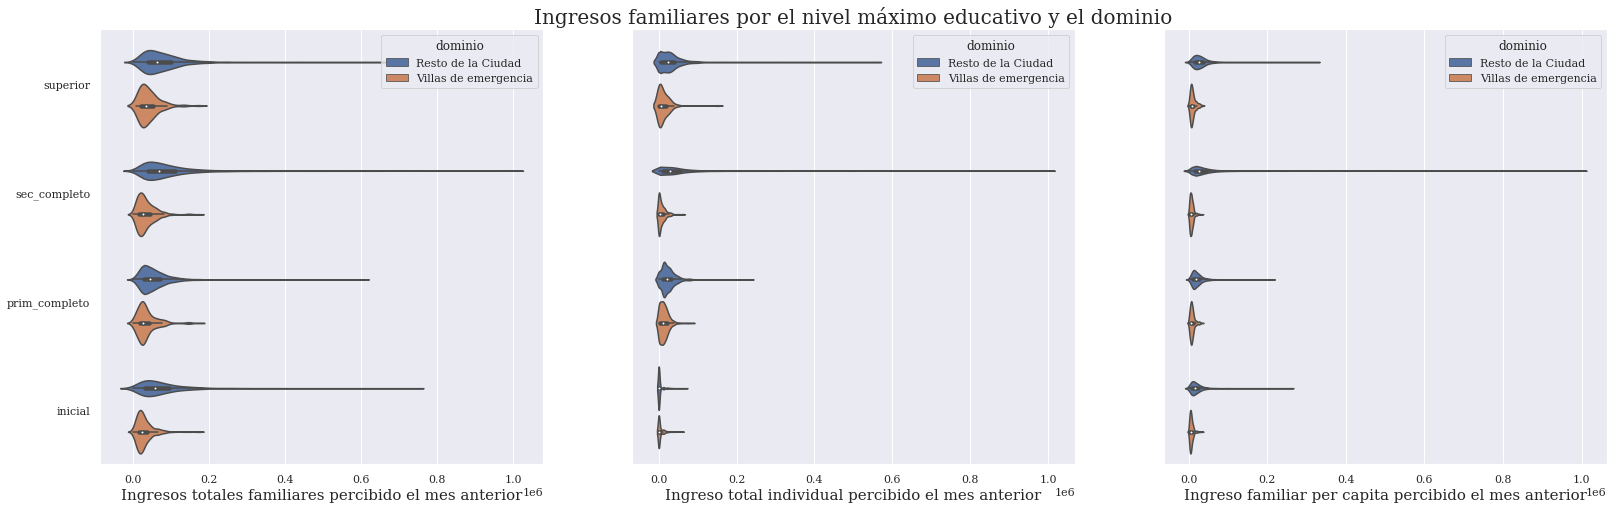
\includegraphics[scale=0.45]{GMul2.png}

            Aquí obtuvimos un descubrimiento interesante: no importa el nivel máximo educativo, los casos que no provienen de villas de emergencia (dominio='villas\_de\_emergencia') obtienen en promedio ingresos más altos en todos los niveles educativos. El alcanzar estudios superiores no parece homogeneizar ambos conjuntos.

        \end{landscape}

        \subsubsection*{Ingresos familiares por comuno y sus nivel educativo}

            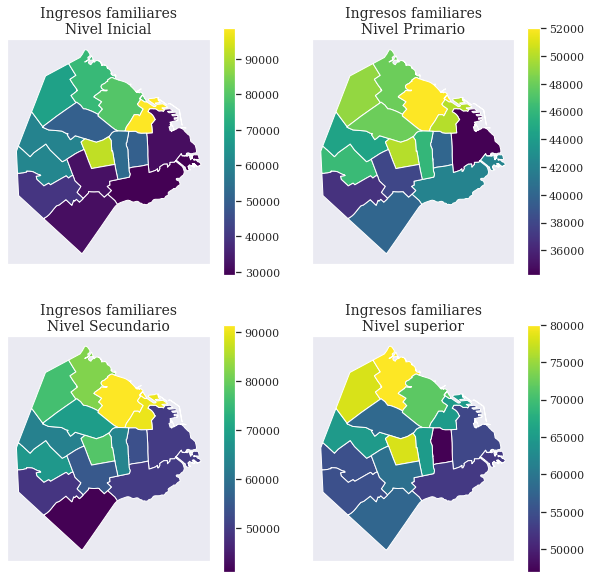
\includegraphics[scale=0.8]{GMul3.png}

            Aquí podemos observar que a medida que avanza el nivel educativo máximo se atenúan levemente las diferencias de ingresos familiares entre comunas. Queda pendiente cruzar estos datos con la edad, para saber si el hecho de incluir a menores de edad está sesgando los valores para nivel inicial, primario y secundario.

\newpage

\section{Modelado de datos}
    
    En primer lugar creamos el ``Target'', recategorizando la variables target en variables numéricas y reagrupamos la variable comuna por regiones para reducir la dimensionalidad.

    Ultilizamos un dataset ``train'' y otro ``test'' $70-30\%$, controlamos sus nulos:
    \begin{center}
        \begin{tabular}{lr}
            Variables con valores nulos en el train: & \\
            & \\
            situacion\_conyugal           & 1 \\
            sector\_educativo             & 1 \\
            afiliacion\_salud             & 3 \\
            años\_escolaridad             & 46\\
            nivel\_max\_educativo          & 733\\
            target                       & 764\\
            Target                       & 764\\
            hijos\_nacidos\_vivos          & 5395
        \end{tabular}
    \end{center}

    \begin{center}
        \begin{tabular}{lr}
            Variables con valores nulos en el test: & \\
            & \\
            lugar\_nacimiento       & 1 \\
            afiliacion\_salud       & 1 \\
            sector\_educativo       & 2 \\
            años\_escolaridad       & 16\\
            nivel\_max\_educativo   & 321\\
            target                  & 332\\
            Target                  & 332\\
            hijos\_nacidos\_vivos     & 2389\\
        \end{tabular}
    \end{center}

    \subsection{División del train y el test}

        \subsubsection{Train}

        \subsubsection*{Tratamiento de Nulos}

            \begin{itemize}
                \item En la variable años\_escolaridad reemplazamos los nulos con la mediana por comuna y sexo.
                \item En las variables lugar\_nacimiento, situacion\_conyugal,afiliacion\_salud, secto\_educativo, hijos\_nacidos\_vivos, reemplazamos los nulos con sus modas respectivas.
                \item Como no podemos reemplazar los nulos del target del train, los eliminamos.
                \item Y además, como ya no la vamos a utilizar tambien eliminamos la variable nivel\_max\_educativo.
            \end{itemize}
            
        \subsubsection*{Borrado de Variables}
            
            Hay muchas variables que consideramos que no es necesario sumarlas al algoritmo de clasificacion dado que brindan información repetida o que no suma para la clasificación. A continuación se comparten las categoria que se descartarán para correr el algoritmo.
            
            \begin{itemize}
                \item \textbf{id:} no suma información para la clasificación,
                \item \textbf{nhogar:} no suma información para la clasificación,
                \item \textbf{parentesco\_jefe:} no suma información para la clasificación,
                \item \textbf{miembro:} no suma información para la clasificación,
                \item \textbf{num\_miembro\_padre:} no suma información para la clasificación,
                \item \textbf{num\_miembro\_madre:} no suma información para la clasificación,
                \item \textbf{cat\_ocupacional:} brinda la misma información que estado\_ocupacional,
                \item \textbf{calidad\_ingresos\_lab:} brinda la misma información que ingreso\_total\_lab,
                \item \textbf{calidad\_ingresos\_no\_lab:} brinda la misma información que ingreso\_total\_no\_lab,
                \item \textbf{calidad\_ingresos\_totales:} brinda la misma información que ingresos\_totales,
                \item \textbf{calidad\_ingresos\_familiares:} brinda la misma información que ingreso\_familiares,
                \item \textbf{estado\_educativo:} no aporta información para la clasificación,
                \item \textbf{nivel\_actual:} no aporta información para la clasificacion,
                \item \textbf{hijos\_nacidos\_vivos:} brinda la misma información que cant\_hijos\_nac\_vivos,
                \item \textbf{comuna:} variable ya abordada en la variable ``región'',
            \end{itemize}
        
        Las variables: 
        \begin{itemize}
            \item id, hogar, miembro, parentesco\_jefe, num\_miembro\_padre, cat\_ocupacional, 
            
            calidad\_ingresos\_lab, calidad\_ingresos\_no\_lab, calidad\_ingresos\_totales, calidad\_ingresos\_familiares,
            
            hijos\_nacidos\_vivos, estado\_educativo, comuna, nivel\_actual, nivel\_max\_educativo,
        \end{itemize}
        no tienen valor para nuestro analisis, por ello las elimnamos.

        \subsubsection*{Target}

            \subsubsection*{One Hot Encoding}

            Las variables categoricas:
            \begin{itemize}
                \item region, situacion\_conyugal, sector\_educativo, estado\_ocupacional, afiliacion\_salud, lugar\_nacimiento, sexo, dominio,
            \end{itemize}
            las transformamos, entrenandolas para generar el preprocesamiento one hot encoding.
            
            Luego, juntamos el train con las variables categoricas anteriores, por último renombramos algunas variables para que sean más cortas.
            \begin{itemize}
                \item afiliacion\_salud\_Solo obra social: afiliacion\_salud\_solo\_o\_social,
                \item afiliacion\_salud\_Solo plan de medicina prepaga por contratación voluntaria: afiliacion\_salud\_solo\_prepaga,
                \item afiliacion\_salud\_Solo prepaga o mutual via OS: afiliacion\_salud\_solo\_prepaga\_o\_mutual,
                \item afiliacion\_Solo sistema publico: afiliacion\_salud\_solo\_sist\_pub,
                \item situacion\_conyugal\_Separado/a de unión o matrimonio: situacion\_conyugal\_separado
            \end{itemize}
        
            % Quedo muy feo...
            \begin{landscape}
            \subsubsection*{División de X e Y}
                
                Spliteamos los datos en target y features para el test, seleccionando la variable x sin el target y para la variable y el target.

                \resizebox{25cm}{!} {
                \begin{tabular}{lrrrrrrrrrrrrrrrrrrrrrrrrrrrrrrrrrr}
                    \toprule
                    &  region\_centro &  region\_norte &  region\_oeste &  region\_sur &  situacion\_conyugal\_Casado/a &  situacion\_conyugal\_Divorciado/a &  situacion\_conyugal\_No corresponde &  situacion\_conyugal\_Separado/a de unión o matrimonio &  situacion\_conyugal\_Soltero/a &  situacion\_conyugal\_Unido/a &  situacion\_conyugal\_Viudo/a &  sector\_educativo\_Estatal/publico &  sector\_educativo\_No corresponde &  sector\_educativo\_Privado no religioso &  sector\_educativo\_Privado religioso &  estado\_ocupacional\_Desocupado &  estado\_ocupacional\_Inactivo &  estado\_ocupacional\_Ocupado &  afiliacion\_salud\_Otros &  afiliacion\_salud\_Solo obra social &  afiliacion\_salud\_Solo plan de medicina prepaga por contratación voluntaria &  afiliacion\_salud\_Solo prepaga o mutual via OS &  afiliacion\_salud\_Solo sistema publico &  lugar\_nacimiento\_CABA &  lugar\_nacimiento\_Otra provincia &  lugar\_nacimiento\_PBA excepto GBA &  lugar\_nacimiento\_PBA sin especificar &  lugar\_nacimiento\_Pais limitrofe &  lugar\_nacimiento\_Pais no limitrofe &  lugar\_nacimiento\_Partido GBA &  sexo\_Mujer &  sexo\_Varon &  dominio\_Resto de la Ciudad &  dominio\_Villas de emergencia \\
                    \midrule
                    0 &            1.0 &           0.0 &           0.0 &         0.0 &                          0.0 &                              0.0 &                                0.0 &                                                0.0 &                           0.0 &                         1.0 &                         0.0 &                               0.0 &                              1.0 &                                    0.0 &                                 0.0 &                            0.0 &                          0.0 &                         1.0 &                     0.0 &                                1.0 &                                                0.0 &                                            0.0 &                                    0.0 &                    0.0 &                              0.0 &                               0.0 &                                   0.0 &                              0.0 &                                 0.0 &                           1.0 &         0.0 &         1.0 &                         1.0 &                           0.0 \\
                    1 &            0.0 &           0.0 &           0.0 &         1.0 &                          0.0 &                              0.0 &                                0.0 &                                                0.0 &                           0.0 &                         1.0 &                         0.0 &                               0.0 &                              1.0 &                                    0.0 &                                 0.0 &                            0.0 &                          0.0 &                         1.0 &                     0.0 &                                1.0 &                                                0.0 &                                            0.0 &                                    0.0 &                    0.0 &                              0.0 &                               0.0 &                                   0.0 &                              1.0 &                                 0.0 &                           0.0 &         0.0 &         1.0 &                         0.0 &                           1.0 \\
                    2 &            0.0 &           0.0 &           1.0 &         0.0 &                          0.0 &                              0.0 &                                0.0 &                                                0.0 &                           0.0 &                         1.0 &                         0.0 &                               0.0 &                              1.0 &                                    0.0 &                                 0.0 &                            0.0 &                          0.0 &                         1.0 &                     0.0 &                                0.0 &                                                0.0 &                                            1.0 &                                    0.0 &                    1.0 &                              0.0 &                               0.0 &                                   0.0 &                              0.0 &                                 0.0 &                           0.0 &         1.0 &         0.0 &                         1.0 &                           0.0 \\
                    3 &            1.0 &           0.0 &           0.0 &         0.0 &                          1.0 &                              0.0 &                                0.0 &                                                0.0 &                           0.0 &                         0.0 &                         0.0 &                               0.0 &                              1.0 &                                    0.0 &                                 0.0 &                            0.0 &                          0.0 &                         1.0 &                     1.0 &                                0.0 &                                                0.0 &                                            0.0 &                                    0.0 &                    1.0 &                              0.0 &                               0.0 &                                   0.0 &                              0.0 &                                 0.0 &                           0.0 &         0.0 &         1.0 &                         1.0 &                           0.0 \\
                    4 &            0.0 &           0.0 &           1.0 &         0.0 &                          0.0 &                              0.0 &                                0.0 &                                                0.0 &                           0.0 &                         1.0 &                         0.0 &                               0.0 &                              1.0 &                                    0.0 &                                 0.0 &                            0.0 &                          0.0 &                         1.0 &                     0.0 &                                0.0 &                                                0.0 &                                            0.0 &                                    1.0 &                    0.0 &                              0.0 &                               0.0 &                                   0.0 &                              1.0 &                                 0.0 &                           0.0 &         1.0 &         0.0 &                         0.0 &                           1.0 \\
                    \bottomrule \\
                \end{tabular} }
            \end{landscape}
        

        \subsubsection{Test}
            
            \subsubsection*{Tratamiento de nulos}

            Para tratar los nulos del test:
            \begin{itemize}
                \item reemplazamoslos nulos de la variable años\_escolaridad con la mediana por comuna,
                \item para las variables lugar\_nacimiento, situacion\_conyugal, afiliacion\_salud, los completamos con sus respectivas medianas,
                \item eliminamos todos los nulos del target,
                \item y por ultimo eliminamos todas la variables que no nos aportan al analisis:
                \begin{itemize}
                    \item id, nhogar, miembro, parentesco\_jefe, num\_miembro\_padre, num\_miembro\_madre', cat\_ocupacional,
                    
                    calidad\_ingresos\_lab, calidad\_ingresos\_no\_lab, calidad\_ingresos\_totales, calidad\_ingresos\_familiares, 
                    
                    hijos\_nacidos\_vivos, estado\_educativo, comuna, nivel\_actual, nivel\_max\_educativo.
                \end{itemize}
            \end{itemize}

            \subsubsection*{One hot encoding}

                Como la primera parte del encoding ya esta hecha para el train, repetimos para el test, con las mismas categoricas.
            
            \subsubsection*{División de X e Y}

                Nuevamente, pero ahora para el test dividimos la variable X (sin el target) y la variable Y para el target. 
    \subsection{Árbol de decisión}

        Utilizamos el árbol de decisiones para casificaciones, con sus parametros default. Y modelamos para el train.
\end{document}